
\section{Notation and Required Definitions}

In this section, we formally describe the notation and definitions 
used in the rest of the paper.  Readers
familiar with polyhedral libraries such as the Integer Set Library
(ISL)~\cite{verdoolaege_isl:_2010} or Omega~\cite{omega} will be familiar with these
concepts and may skip to the next section.


\paragraph{Presburger formula}

We use an EBNF (Extended Backus-Naur Form) grammar to define Presburger formulas.
\[
\begin{array}{lcl}
\pgrammar{formula} & \gets &  \pgrammar{formula} \wedge \pgrammar{formula} \\ 
        & & ~|~ \pgrammar{formula} \vee   \pgrammar{formula} \\
        & & ~|~ \neg \pgrammar{formula} 
        ~|~ \exists \pgrammar{var}. \pgrammar{formula} \\
        & & ~|~ \forall \pgrammar{var}. \pgrammar{formula}
        ~|~ \pgrammar{atom} \\
                            
\pgrammar{atom} & \gets &  \pgrammar{term} \pgrammar{relop} \pgrammar{term}
                            \\
\pgrammar{term} & \gets &     \pgrammar{numeral}
        ~|~ \pgrammar{term} + \pgrammar{term} \\
        & & ~|~ -\pgrammar{term} \\
        & & ~|~ \pgrammar{numeral} * \pgrammar{term}
        ~|~ \pgrammar{var}
                            \\
\pgrammar{relop} & \gets &    <
        ~|~ \leq
                            ~|~ =
                            ~|~ >
                            ~|~ \geq
                            \\
\pgrammar{var} & \gets &      x
                            ~|~ y
                            ~|~ z
                            ~|~ \dots
                            \\
\pgrammar{numeral} & \gets &  0
                            ~|~ 1
                            ~|~ 2
                            ~|~ \dots
                            \\
\end{array}
\]

Note that $\pgrammar{numeral} * \pgrammar{term}$ is not a general multiplication operator;
it is a shortcut for $\pgrammar{term}+\dots+\pgrammar{term}$.

Presburger arithmetic is used mainly because it is a decidable arithmetic.
That is, there exists an algorithm which decides whether an arbitrary Presburger formula is true (valid) or not, which is important for many polyhedral operations.


\paragraph{Quasi-Affine Constraints}
\label{qaffine}

A \emph{quasi-affine constraint} is a constraint over integer values and integer variables involving only the operators \lstinline{+}, \lstinline{-}, $\times$, \lstinline{/}, \lstinline{mod}, \lstinline{&&}, \lstinline{||}, \lstinline{<}, \lstinline{<=}, \lstinline{>}, \lstinline{>=}, \lstinline{==}, \lstinline{!=}, and the ternary \lstinline{?:} operator, where the second argument of \lstinline{/} and \lstinline{mod} must be a (positive) integer literal, and where at
least one of the arguments of $\times$
must be a constant expression.
An example of a quasi-affine constraint for a statement in a loop nest is $10\times i+j+n>0$, where $i$ and $j$ are loop iterators and $n$ is a
\emph{symbolic constant} (i.e., a variable that has an unknown but fixed value for the duration of
an execution).  An example of a non-quasi-affine constraint is $i \times i>0$, because we require one of the arguments be a constant.

\paragraph{Integer Sets}

An \emph{integer set} is a set of integer tuples from $\mathbb{Z}^d$ that can be specified using  quasi-affine constraints. $d$ is the dimensionality of the set (the number of integers in each tuple) and a d-tuple is represented as $[a_1, a_2, \dots, a_d]$.  An example of a set of integer tuples is:
$$\{[1,1]; [2,1]; [3,1]; [1,2]; [2,2]; [3,2]\}$$

Instead of listing all the integer tuples of the set, we describe the set using quasi-affine constraints:
$$\{S[i,j]:  1 \leq i \leq 3 \wedge 1 \leq j \leq 2\}$$

\noindent where $i$ and $j$ are the dimensions of the set.
The tuples of a set can optionally have a common name, such as
$S$ in this example.

In general, an integer set has the form
$$S = \{N[\vec{s}] | f(\vec{s}, \vec{p})\}$$

\noindent with $\vec{s}$ representing the integer tuples of
the integer set ($\vec{s} \in \mathbb{Z}^d$), $N$, a common name
for all the tuples $\vec{s}$ usually used as the name of computations, $d$ the dimensionality of the set, $\vec{p} \in \mathbb{Z}^e$ a vector of $e$ parameters and $f(\vec{s}, \vec{p})$ a Presburger formula that evaluates to true, if and only if $\vec{s}$ is an element of $S$ for the given parameters $\vec{p}$.

\subsection{Maps}

A map is a relation between two integer sets.  For example
$$M = \{S1[i,j] \rightarrow S1[i+2,j+2] : 1 \leq i \leq 3 \wedge 1 \leq j \leq 2\}$$

\noindent represents a relation between two sets. The first set
is called the \emph{domain} or the \emph{source}
and the second is called the \emph{range} or the
\emph{sink}.
Figure~\ref{fig:map} shows a graphical representation of
the map $M$.

\begin{figure}[th]
  \centering
  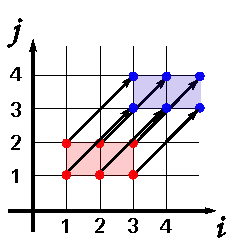
\includegraphics[scale=0.7]{figures/map.pdf}
  \caption{Graphical representation of a map}
  \label{fig:map}
\end{figure}

In general, a map has the form
$$M = \{A[\vec{s}] \rightarrow B[\vec{o}], (\vec{s}, \vec{o}) \in \mathbb{Z}^{d_1}\times\mathbb{Z}^{d_2} | f(\vec{s}, \vec{o}, \vec{p})\}$$

\noindent where $A[\vec{s}]$ represents the domain or the
source and $B[\vec{o}]$ represents the range or the sink.
$d_1$ and $d_2$ are the dimensionalities of $\vec{s}$
and $\vec{o}$, $\vec{p} \in \mathbb{Z}^e$ is a vector of $e$ parameters and $f(\vec{s}, \vec{o}, \vec{p})$ is a Presburger formula that evaluates to true if and only if there is a relation from $\vec{s}$ to $\vec{o}$ in $M$ for the given parameters
$\vec{p}$.
